\input ../../SlidePreamble
\input ../../preamble


\begin{document}

{\Huge
  \centerline{\bf TTIC 31230,  Fundamentals of Deep Learning}
  \vfill
  \centerline{David McAllester, Autumn   2020}
  \vfill
  \centerline{\bf Contrastive Predictive Coding}
  \vfill
  \vfill


\slide{Maximizing Mutual Information}

We consider the distribution on $x$, $y$, $z_x$ and $z_y$ defined by drawing $\tuple{x,y} \sim \pop$, $z_x \sim P_\Phi(z_x|x)$ and $z_y \sim P_\Phi(z_y|y)$.

\vfill
We are interested in optimizing $P_\Phi(z_x|x)$ and $P_\Phi(z_y|y)$ under the following objective.
\vfill
$$\Phi^* = \argmax_{\Phi} \; I_{\pop,\Phi}(z_x,z_y) - \beta (H_{\pop,\Phi}(z_x) + H_{\pop,\Phi}(z_y))$$

\slide{Maximizing Mutual Information}

\begin{eqnarray*}
\Phi^* & = & \argmax_{\Phi} \; I_{\pop,\Phi}(z_x,z_y) - \beta ({\color{red} H}_{\pop,\Phi}(z_x) + {\color{red} H}_{\pop,\Phi}(z_y)) \\
\\
& \geq & \argmax_{\Phi} \; I_{\pop,\Phi}(z_x,z_y) - \beta ({\color{red} \hat{H}}_{\pop,\Phi}(z_x) + {\color{red} \hat{H}}_{\pop,\Phi}(z_y))
\end{eqnarray*}

\vfill
\begin{eqnarray*}
{\color{red} H}_{\pop,\Phi}(z_x) & = & E_{\pop,\Phi}\;-\ln P_{\color{red} \pop,\Phi}(z_x) \\
\\
{\color{red} \hat{H}}_{\pop,\Phi}(z_x) & = & E_{\pop,\Phi}\;-\ln P_{\color{red} \Phi}(z_x) \\
\\
{\color{red} H}_{\pop,\Phi}(z_x) & \leq & {\color{red} \hat{H}}_{\pop,\Phi}(z_x)
\end{eqnarray*}



\slide{Maximizing Mutual Information}

$$\Phi^* = \argmax_{\Phi} \; I_{\pop,\Phi}(z_x,z_y) - \beta (\hat{H}_\Phi(z_x) + \hat{H}_\Phi(z_y))$$

\vfill
It turns out that we can give a lower bound on the mutual information term using {\bf noise contrastive estimation}.

\slide{A Contrastive Lower Bound}

We now give a contrastive lower bound for general mutual information $I(z,w)$ given only the ability to sample from the joint distribution on $z$ and $w$.

\vfill
For $N \geq 2$ let {\color{red} $c_{z,w}$} be the density defined by drawing pairs $(z_1,w_1), \ldots (z_n,w_n)$ from the population
and then constructing the tuple $(i,z_1,\ldots,z_N,w)$ where $i$ is drawn uniformly from $1$ to $N$ and $w = w_i$ is the value of $w$ paired with $z_i$.

\slide{A Constrastive Lower Bound}

{\huge
\begin{eqnarray*}
\Phi^* & = & \argmin_\Phi \;E_{(i,z_1\ldots,z_N,w) \sim c_{z,w}}\;-\ln P_\Phi(i|z_1,\ldots,z_n,w) \\
\\
& = & \argmin_\Phi\;{\cal L}(\Phi) \\
\\
P_\Phi(i|z_1,\ldots z_n,w) & = & \softmax_i\;s_\Phi(z_i,w) \;\;\;\mbox{(required)} \\
\\
I(z,w) & \geq & \ln N - {\cal L}(\Phi)
\end{eqnarray*}
}

See Chen et al., On Variational Bounds of Mutual Information, May 2019.

\slide{Forcing $z_x$ and $z_y$ to be Useful}

In the objective

$$\Phi^* = \argmax_{\Phi} \; I_{\pop,\Phi}(z_x,z_y) - \beta ({\color{red} H_{\pop,\Phi}(z_x)} + {\color{red} H_{\pop,\Phi}(z_y)})$$


the limitation on the entropy of $z_x$ and $z_y$ block the trivial solution of $z_x = x$ and $z_y = y$.


\vfill
CPC applications have used an alternative.

\slide{Forcing $z_x$ and $z_y$ to be Useful}

\begin{eqnarray*}
\Phi^* & = & \argmin_\Phi \;E_{(i,z_x^1\ldots,z_x^n,z_y) \sim c_{z_x,z_y}}\;-\ln P_\Phi(i|z_x^1,\ldots,z_x^n,z_y)
\end{eqnarray*}

\begin{eqnarray*}
P_\Phi(i|z_x^1,\ldots,z_x^n,z_y) & = & \softmax_i\;{\color{red} z_y^\top z_x^i}
\end{eqnarray*}


\vfill
Requiring that the score be a simple inner product blocks $z_x = x$ and $z_y = y$ and forces
$z_x$ and $z_y$ to carry the information in a linearly extractible way.

\slide{Contrastive Predictive Coding for Speech}

{\huge

\centerline{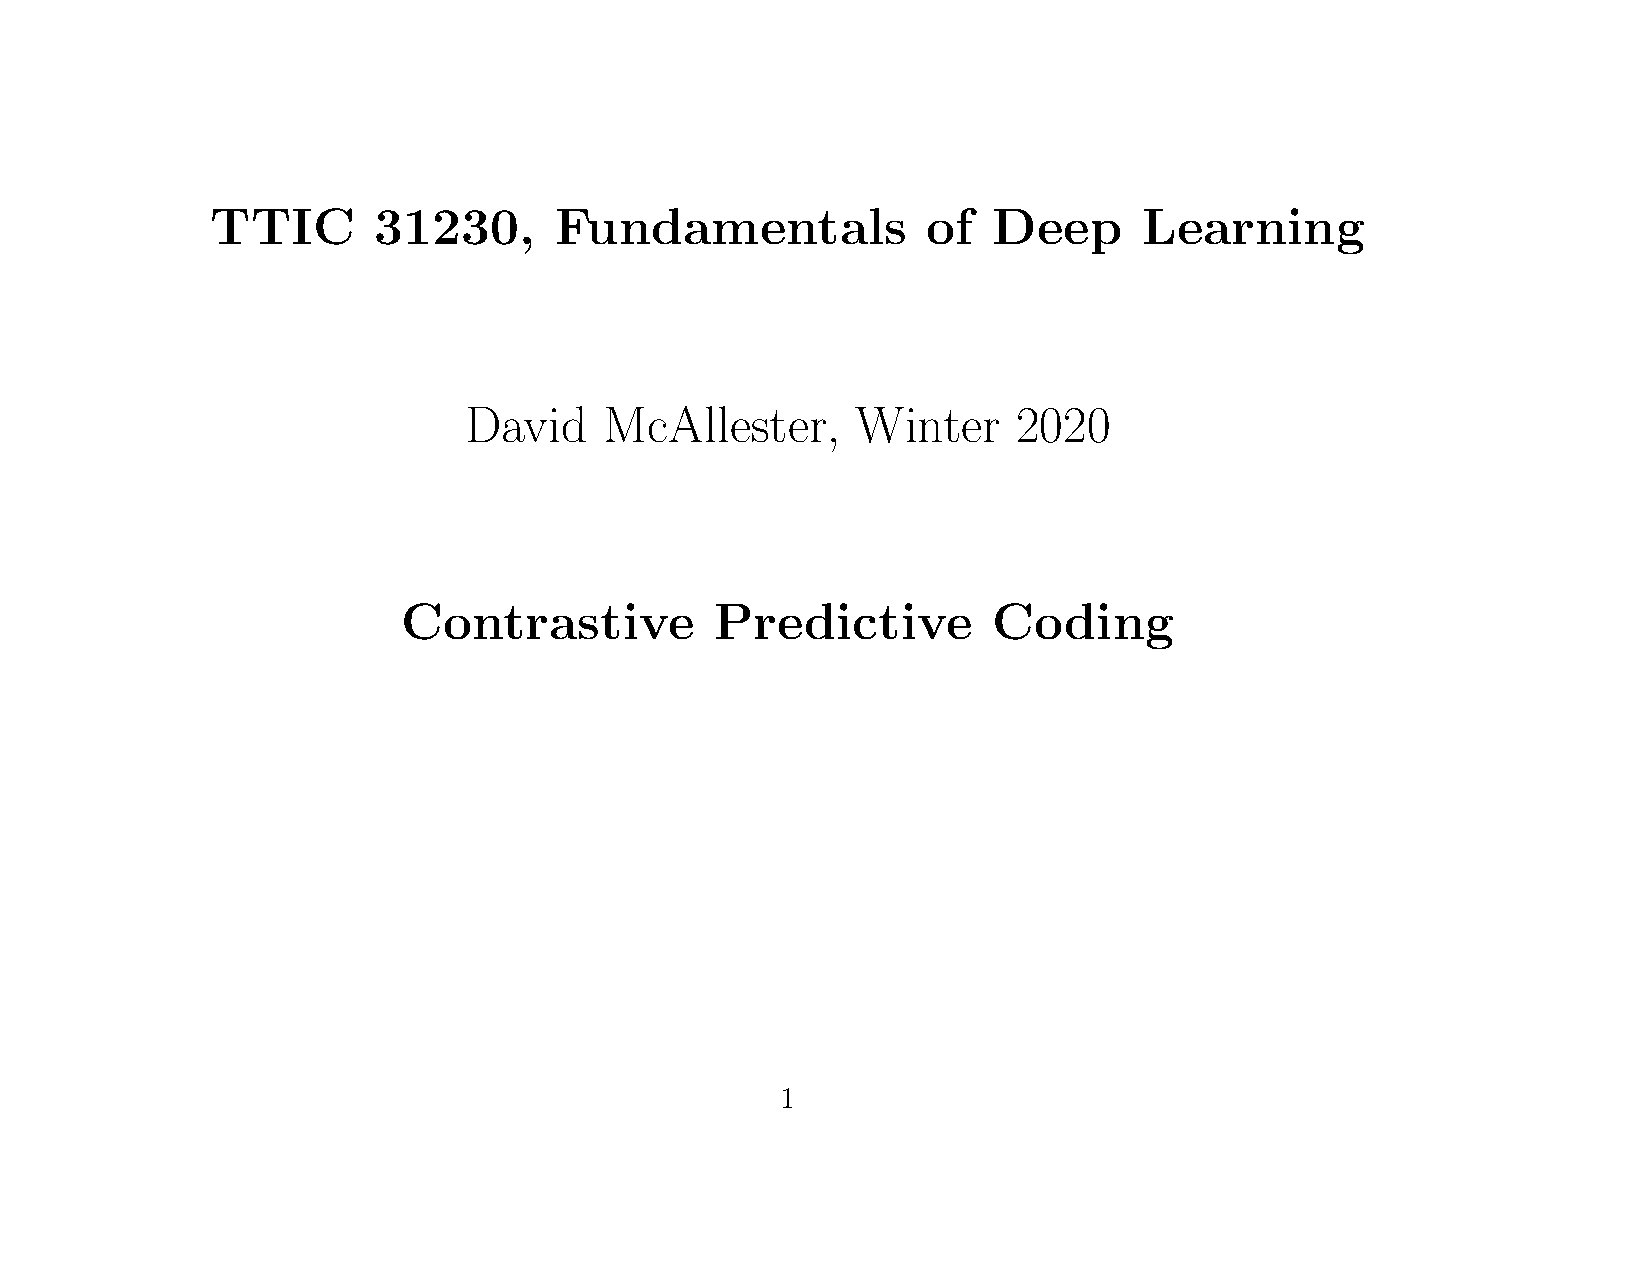
\includegraphics[width = 5 in]{\images/CPC}}

\centerline{van den Oord et al., 2018}

\vfill

We seek to train an auto-regressive $g_{ar}$ and encoder $g_{env}$ by
\begin{eqnarray*}
g_{ar}^*,g_{enc}^* & = & \argmax_{g_{ar},g_{enc}}\;E_t  \;\sum_{k=1}^K \;I(c_t,z_{t+k})
\end{eqnarray*}
}

\vfill
The training maximizes the contrastive lower bound on $I(c_t,z_{t+k})$

\slide{Contrastive Predictive Coding for Images}

(SimCLR:) A Simple Framework for Contrastive Learning of Visual Representations, Chen et al., Feb. 2020 (self-supervised leader as of February, 2020).

\vfill
They construct a distribution on pairs $\tuple{x,y}$ defined by drawing an image from ImageNet and then drawing $x$ and $y$ as random ``augmentations'' (modifications) of the image.

\vfill
The training maximizes the contrastive lower bound on $I(x,y)$.

\slide{Contrastive Predictive Coding for Images}

A resulting feature map $z_\Phi$ on images is extracted from this training.

\vfill
The feature map $z_\Phi$ is tested by using a {\color{red} linear} classifier for ImageNet based on these features.

\slide{SimCLR}

\centerline{\includegraphics[height=5.2 in]{\images/SimCLR}}

\slide{END}

}
\end{document}

